\section{Referêncial Teórico}

\subsection{Relação Anual de Informações Sociais (RAIS)}

A gestão governamental do setor do trabalho conta com o importante instrumento de coleta de dados denominado de Relação Anual de Informações Sociais - RAIS (Relação Anual de Informações Sociais) \cite{Sobre_a_RAIS}. Instituída pelo Decreto nº 76.900, de 23 de dezembro de 1975 e regida atualmente pelo Decreto nº 10.854, de 10 de novembro de 2021, a RAIS (Relação Anual de Informações Sociais) tem por objetivo: 

\begin{itemize}
	\item O suprimento às necessidades de controle da atividade trabalhista no País
	\item O provimento de dados para a elaboração de estatísticas do trabalho
	\item A disponibilização de informações do mercado de trabalho às entidades governamentais.
\end{itemize}

\subsection{A pandemia da COVID-19}

A pandemia da COVID-19 A partir de 2020, se iniciou uma nova crise de proporções globais, provocada pelo coronavírus (Sars-Cov-2). Em 31 de dezembro de 2019, a Organização Mundial de Saúde – OMS foi alertada sobre o surgimento do vírus em Wuhan, na República Popular da China; entendido primeiramente como um caso de pneumonia, posteriormente descobriu-se a existência de um vírus específico. Em 11 de março de 2020, caracterizou-se a pandemia da COVID-19, que provocou milhões de mortes ao redor do mundo. 

Se espalhando em escala global, a doença foi enfrentada de diversas maneiras, a depender da posição política das lideranças governamentais e do alinhamento com medidas sanitárias recomendadas pela OMS. Para evitar o aumento da contaminação, medidas de prevenção foram adotadas, como o uso de equipamentos de proteção individual – EPI, distanciamento e isolamento social. No Brasil, esse processo incluiu uma disputa judicial entre o governo federal e os governos estaduais. O primeiro foi contrário às medidas de isolamento social impostas por estados e municípios, com o argumento da necessidade de proteção da economia e dos empregos. O Supremo Tribunal Federal – STF deu autonomia relativa a estados e municípios e permitiu a ação do governo federal especificamente para reforçar ações protetivas.

\subsection{Cross Industry Standard Process for Data Mining (CRISP-DM)}

Analisaremos os dados da base de Relação Anual de Informações Sociais – RAIS usando a metodologia CRISP-DM \cite{chapman2000crisp}. O CRISP-DM (Cross Industry Standard Process for Data Mining) é um processo padrão para mineração de dados.

O CRISP-DM envolve um ciclo faseado para um projeto ou pesquisa de mineração de dados (Figura \ref{fig1})):

\begin{figure}[htbp]
	\centerline{
		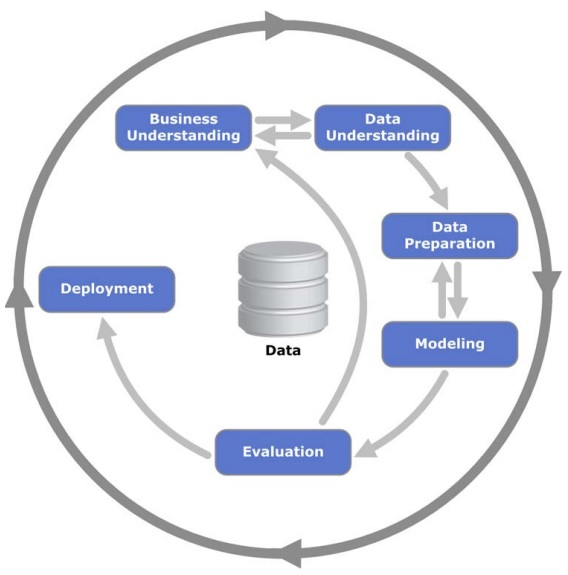
\includegraphics[width=80mm,scale=0.8]{assets/crispdm.jpg}
	}
	\caption{Phases of the CRISP-DM Process Model}
	\label{fig1}
\end{figure}

\begin{enumerate}
	\item Compreensão do negócio: nesta etapa, iremos entender o contexto do problema apresentado e as necessidades apontadas pelo setor público.
	\item Compreensão dos dados: nesta etapa, os dados do RAIS serão coletados e examinados para identificar problemas de qualidade e verificar se eles são adequados para atender aos objetivos da pesquisa.
	\item Preparação dos dados: nesta etapa, os dados da RAIS serão preparados para análise, o que pode incluir a limpeza de dados, a transformação de variáveis e a seleção de subconjuntos de dados relevantes. 
	\item Modelagem: nesta etapa, serão aplicados modelos estatísticos ou de aprendizado de máquina para identificar padrões nos dados da RAIS, bem como relações entre variáveis.
	\item Avaliação: nesta etapa, os resultados da modelagem serão avaliados para verificar se eles atendem aos objetivos da pesquisa, isto é, se eles fornecem informações úteis.
	\item Implantação: nesta etapa final, os resultados serão apresentados e as hipóteses confirmadas ou refutadas.     	      	      	      	      	      
\end{enumerate}
